\chapter{\ifproject%
\ifenglish Project Structure and Methodology\else โครงสร้างและขั้นตอนการทำงาน\fi
\else%
\ifenglish Project Structure\else โครงสร้างของโครงงาน\fi
\fi
}

ในบทนี้จะกล่าวถึงหลักการ และการออกแบบระบบ

\makeatletter

% \renewcommand\section{\@startsection {section}{1}{\z@}%
%                                    {13.5ex \@plus -1ex \@minus -.2ex}%
%                                    {2.3ex \@plus.2ex}%
%                                    {\normalfont\large\bfseries}}

\makeatother
%\vspace{2ex}
% \titleformat{\section}{\normalfont\bfseries}{\thesection}{1em}{}
% \titlespacing*{\section}{0pt}{10ex}{0pt}

\section{หลักการทำงานของระบบ}

% \begin{figure}
% \begin{center}
% 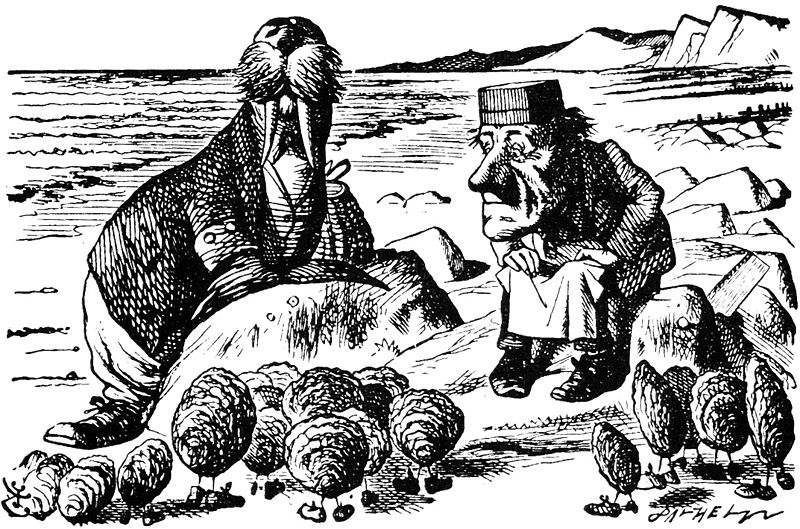
\includegraphics{images/800px-Briny_Beach.jpg}
% \end{center}
% \caption[Poem]{The Walrus and the Carpenter}
% \label{fig:walrus}
% \end{figure}

\subsection{ภาพรวมของระบบ (System Overview)}
  
ภาพรวมการทํางานของระบบนี้ จะมีส่วนการทํางานหลัก ๆ ดังนี้

• ระบบการอัพโหลดและการทํานายรอยโรคในช่องปากโดย AI

• ระบบประวัติการอัพโหลดและการทํานายรอยโรคในช่องปากสําหรับแต่ละผู้ใช้งาน

• ระบบการวงรอยโรคสําหรับทันตแพทย์(Annotation)

• ระบบการแพทย์ทางไกล (Telemedicine) สําหรับให้ความคิดเห็นระหว่างทันตแพทย์ผู้เชี่ยวชาญกับ
ทันตแพทย์ทั่วไป, อาสาสมัครสาธารณสุขประจําหมู่บ้าน, ทันตบุคลากรและผู้ใช้ทั่วไป

• ระบบจัดการผู้ใช้งาน (User Management) และระบบติดตามผู้ใช้งาน (User Tracking)

• ระบบจัดการข้อมูล (Data Management)

\subsection{โครงสร้างฐานข้อมูล (Database Schema)}

Database diagram ของระบบของเรา ได้ทําการเเบ่งผู้ใช้งานเป็น 2 ส่วนหลัก ๆ คือ patients เเละ
users โดย patients คือ คนไข้ทั่วไป เเละ users คือกลุ่มทันตเเพทย์ พนักงานสาธารณสุขเเละผู้ดูแลระบบ
รวมถึงอสม.

ตาราง comment ระบบจะให้เฉพาะทันตเเพทย์ที่มีใบ NL ในการ comment ข้อมูลเท่านั้น โดยสามารถ
บอกได้ว่าเห็นด้วยหรือไม่เห็นด้วย ด้วยเหตุผลอย่างไร

ตาราง users log เป็น table ที่สามารถดูได้เฉพาะ user ที่เป็นผู้ดูแลระบบเท่านั้น โดยจะบอกเกี่ยวกับ
action ของผู้ใช้งานทุกคนว่า ได้มีinteract กับระบบอย่างไรบ้าง โดยที่ action จะมีlogin, logout , delete
รวมถึว action ที่สําคัญต่าง ๆ ไม่ว่าจะเป็น delete user, การ uplaod image โดยเก็บเป็น unixtime เพื่อ
ทําให้ง่ายต่อการ parse

การเข้ารหัสข้อมูล (Encryption) เนื่องจากระบบของเรามีข้อมูลส่วนตัวมากมายที่เก็บเอาไว้ เราจึงต้อง
ทําการเข้ารหัสข้อมูลตาม requirement ที่เราได้รับมา โดยจะมีfile รูปภาพที่เป็นความลับของคนไข้เเละ
ทําการเข้ารหัส password เพื่อความปลอดภัย

\section{ส่วนเชื่อมต่อระหว่างผู้ใช้งานกับระบบ (User Interface)}

ขอแสดงเฉพาะส่วนที่สำคัญและส่วนที่ผู้จัดทำได้มีส่วนในการพัฒนา
\subsection{ทันตบุคลากรและผู้ใช้ทั่วไป (User)}
\subsubsection{หน้าเข้าสู่ระบบ (Login Page)}
\begin{figure}[H]
    \centering
    
\includegraphics[scale=0.3]{images/login_dent.png}
    \caption{login page}
    \label{fig:login_user}
  \end{figure}

\subsubsection{หน้าลงทะเบียน (Register Page)}

\begin{figure}[H]
    \centering
    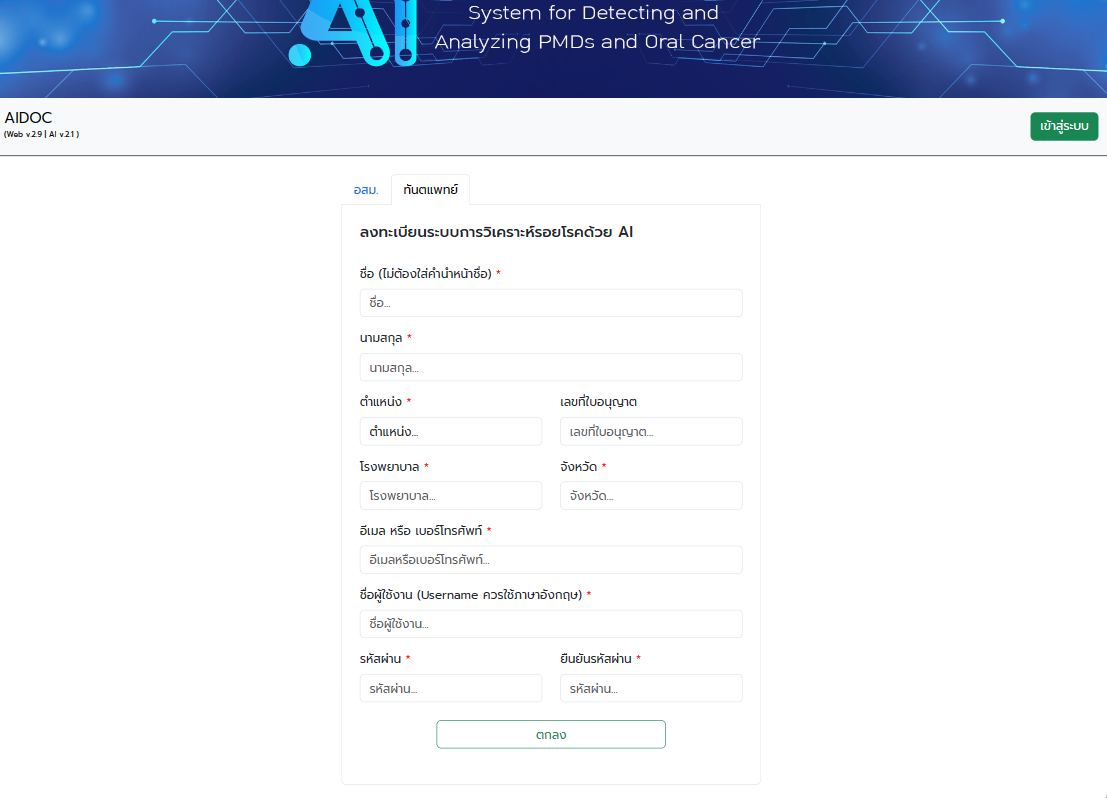
\includegraphics[scale=0.3]{images/register_user.png}
    \caption{register page}
    \label{fig:register_user}
  \end{figure}
\subsubsection{หน้าประวัติการอัพโหลดรูปภาพ (History Page)}

\begin{figure}[H]
  \centering
  \graphicspath{{./images/}}
  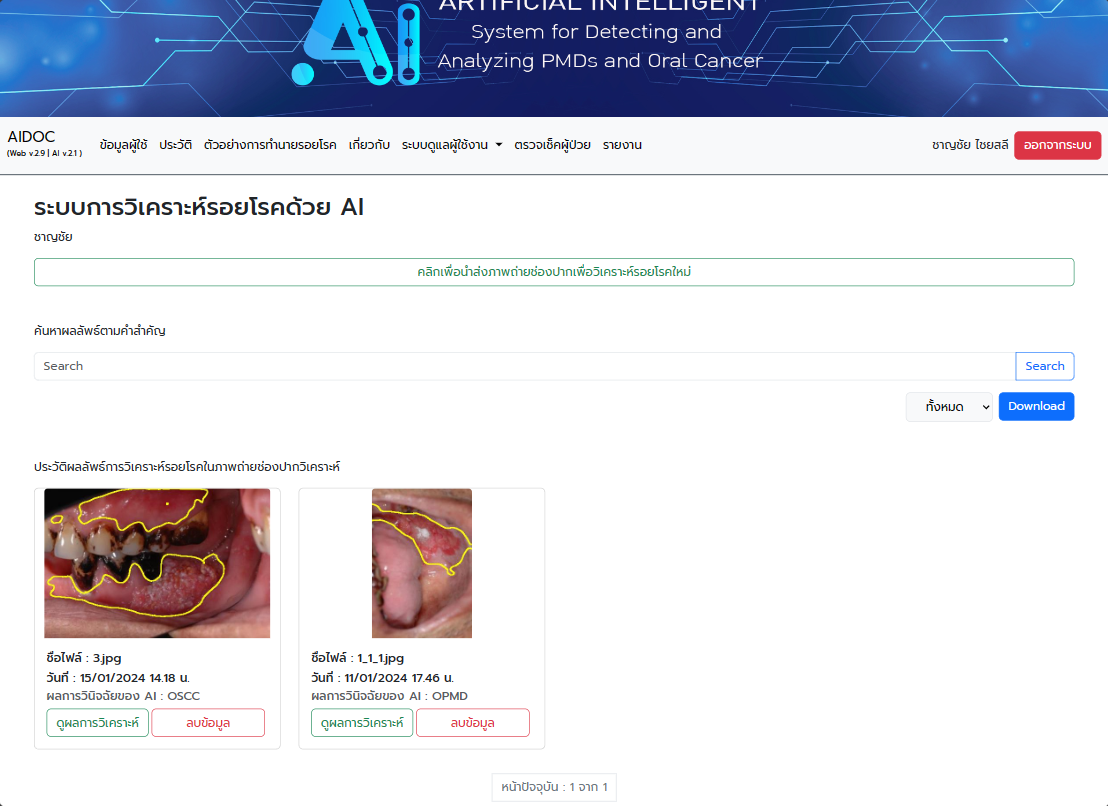
\includegraphics[scale=0.3]{history_user.png}
  \caption{history page}
  \label{fig:history_user}
\end{figure}

\begin{figure}[H]
  \centering
  \graphicspath{{./images/}}
  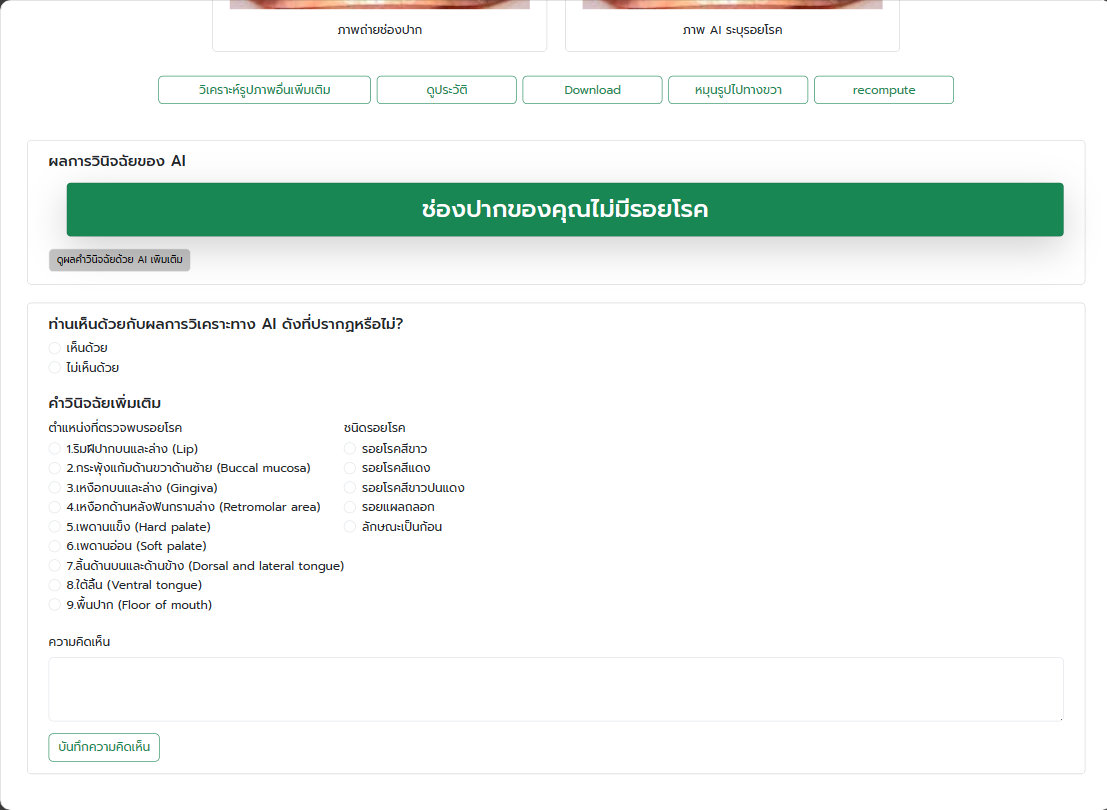
\includegraphics[scale=0.3]{comment_user.png}
  \caption{history page: comment}
  \label{fig:comment_user}
\end{figure}
\subsubsection{หน้าอัพโหลดรูปภาพ (Upload Page)}


\begin{figure}[H]
  \centering
  
\includegraphics[scale=0.3]{images/upload_user.png}
  \caption{upload page}
  \label{fig:upload_user}
\end{figure}

\begin{figure}[H]
  \centering
  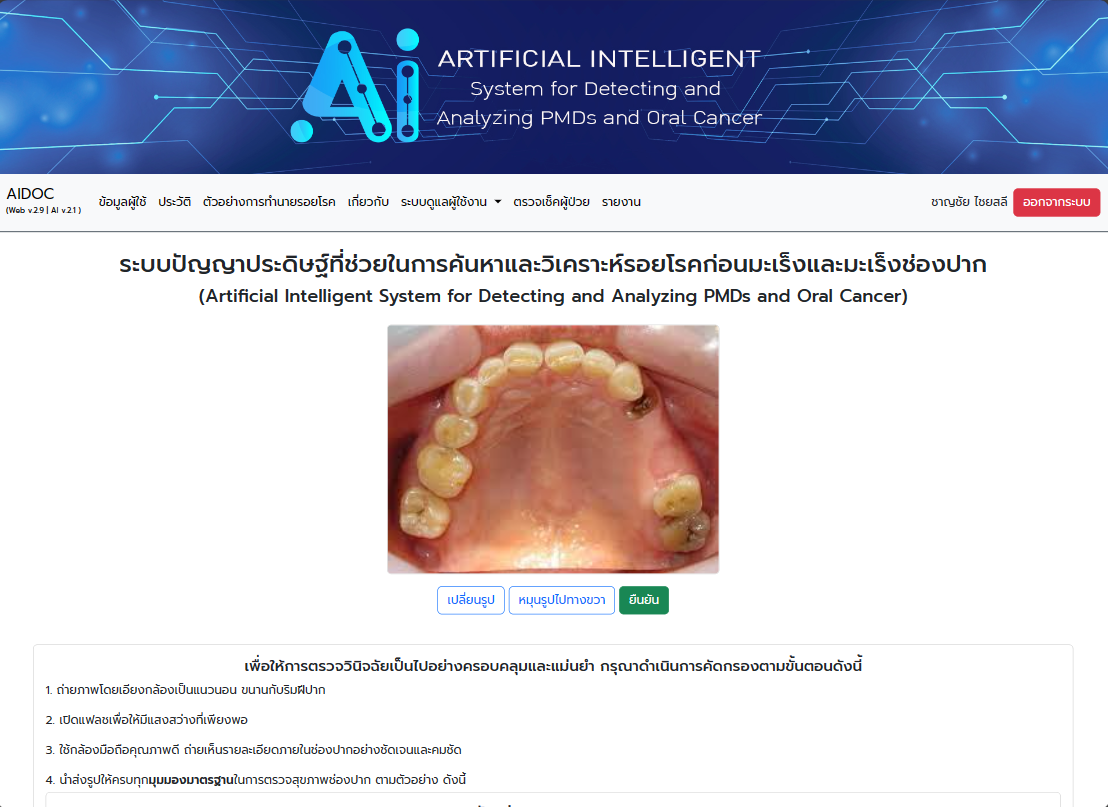
\includegraphics[scale=0.3]{images/preview_user.png}
  \caption{preview page}
  \label{fig:preview_user}
\end{figure}

\begin{figure}[H]
  \centering
  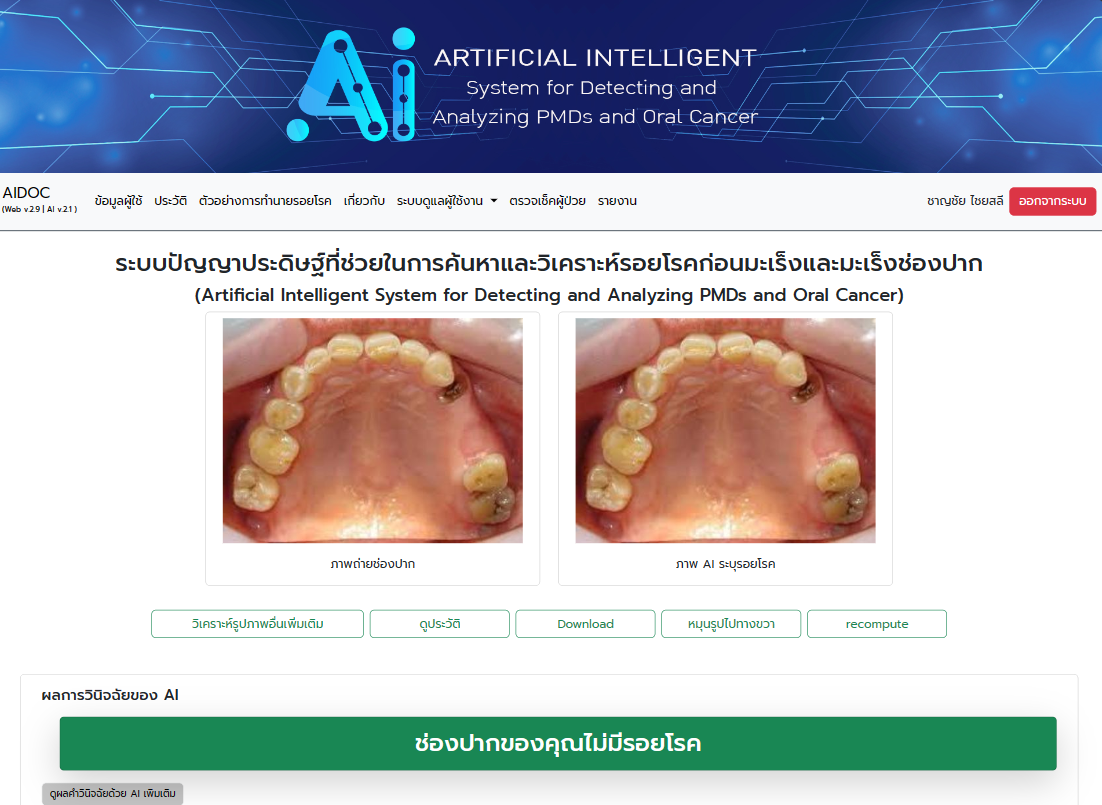
\includegraphics[scale=0.3]{images/upload_complete_user.png}
  \caption{uploaded page}
  \label{fig:upload_complete_user}
\end{figure}

\subsubsection{หน้าประวัติการส่งรูปจากผู้ป่วย (Checkup Page)}

\begin{figure}[H]
  \centering
  \graphicspath{{./images/}}
  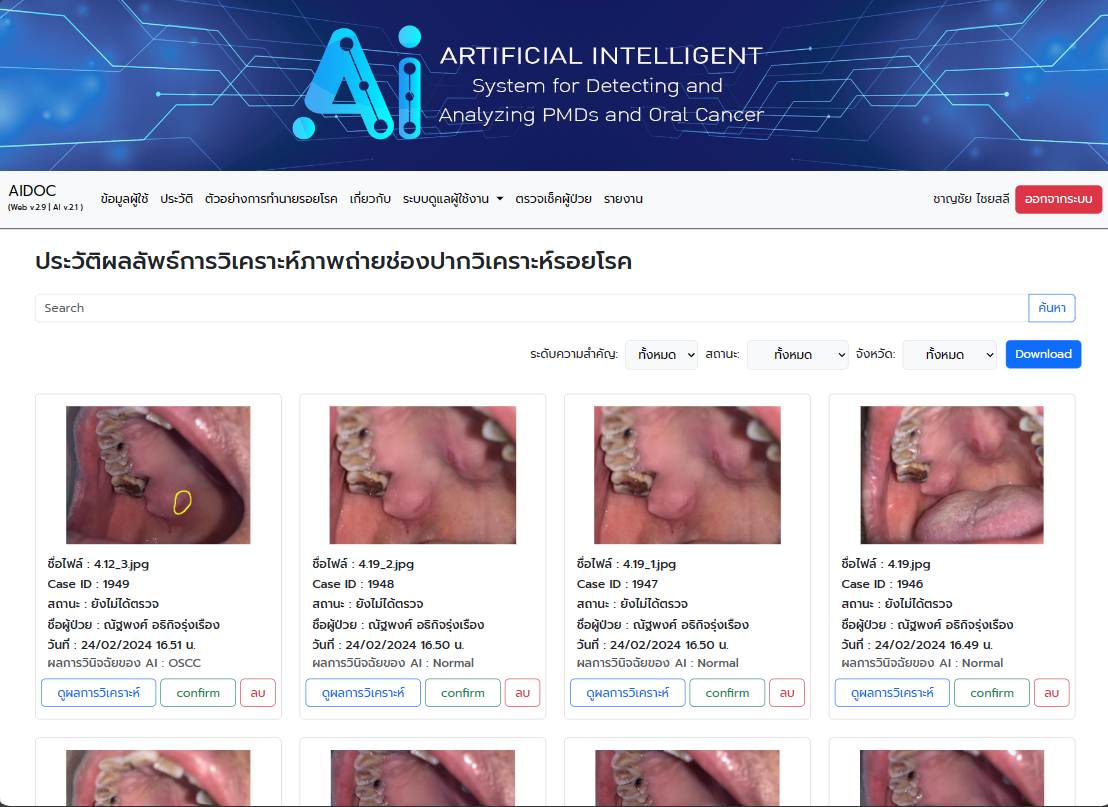
\includegraphics[scale=0.3]{checkup_user.png}
  \caption{checkup page}
  \label{fig:checkup_user}
\end{figure}
\subsubsection{หน้าตรวจเช็คผู้ป่วย (Checking Page)}
\begin{figure}[H]
  \centering
  \graphicspath{{./images/}}
  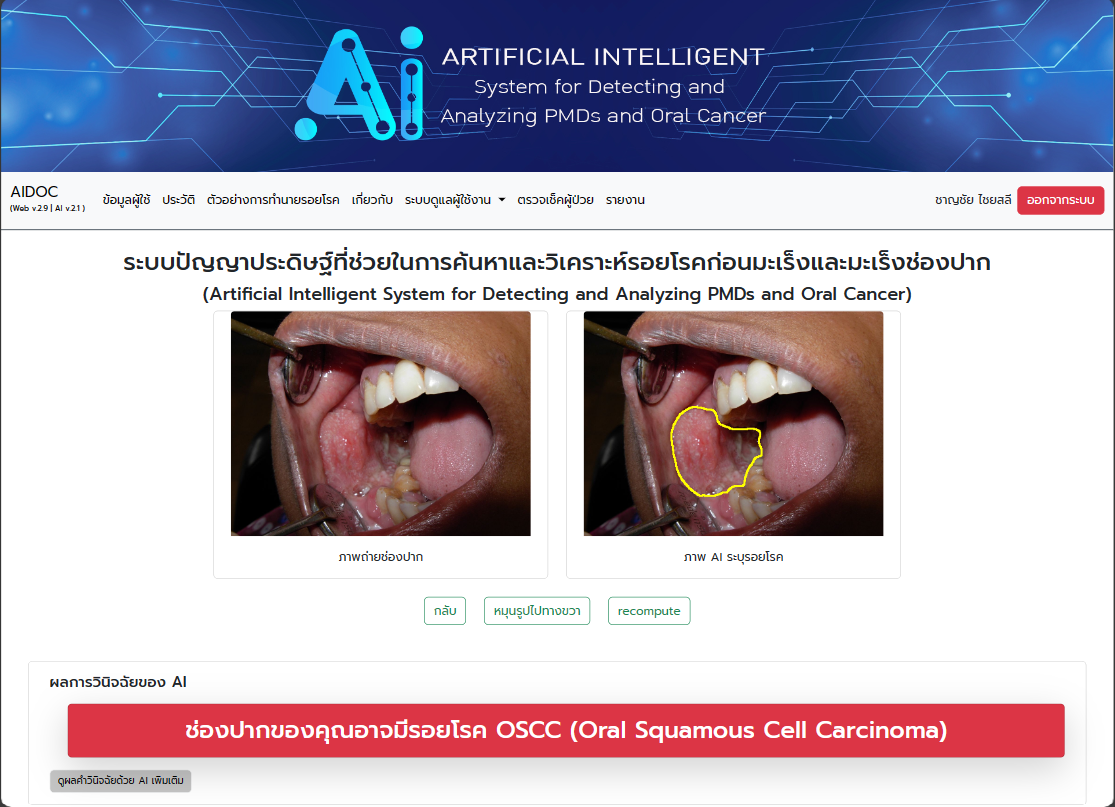
\includegraphics[scale=0.3]{checking_user.png}
  \caption{checking page}
  \label{fig:checking_user}
\end{figure}

\begin{figure}[H]
  \centering
  \graphicspath{{./images/}}
  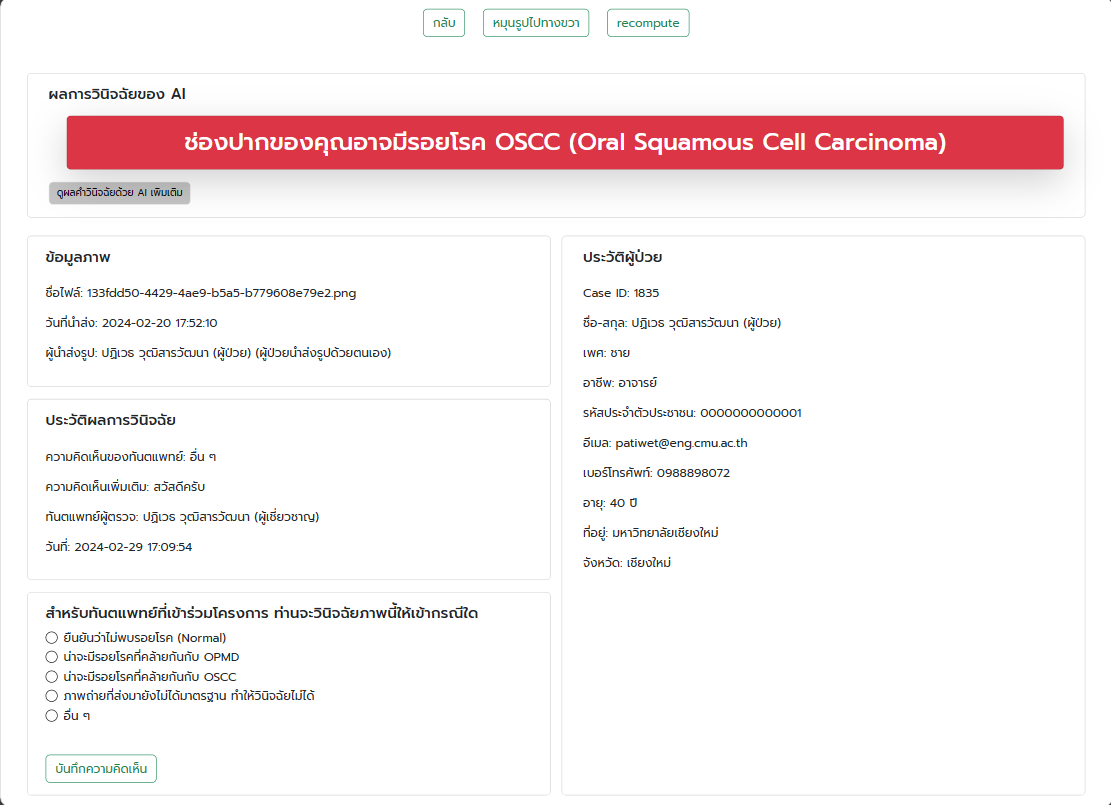
\includegraphics[scale=0.3]{dentist_comment_user.png}
  \caption{checking page: comment}
  \label{fig:dentist_comment_user}
\end{figure}

\subsubsection{หน้ารายงานผลการส่งภาพ (Report Page)}

\begin{figure}[H]
  \centering
  \graphicspath{{./images/}}
  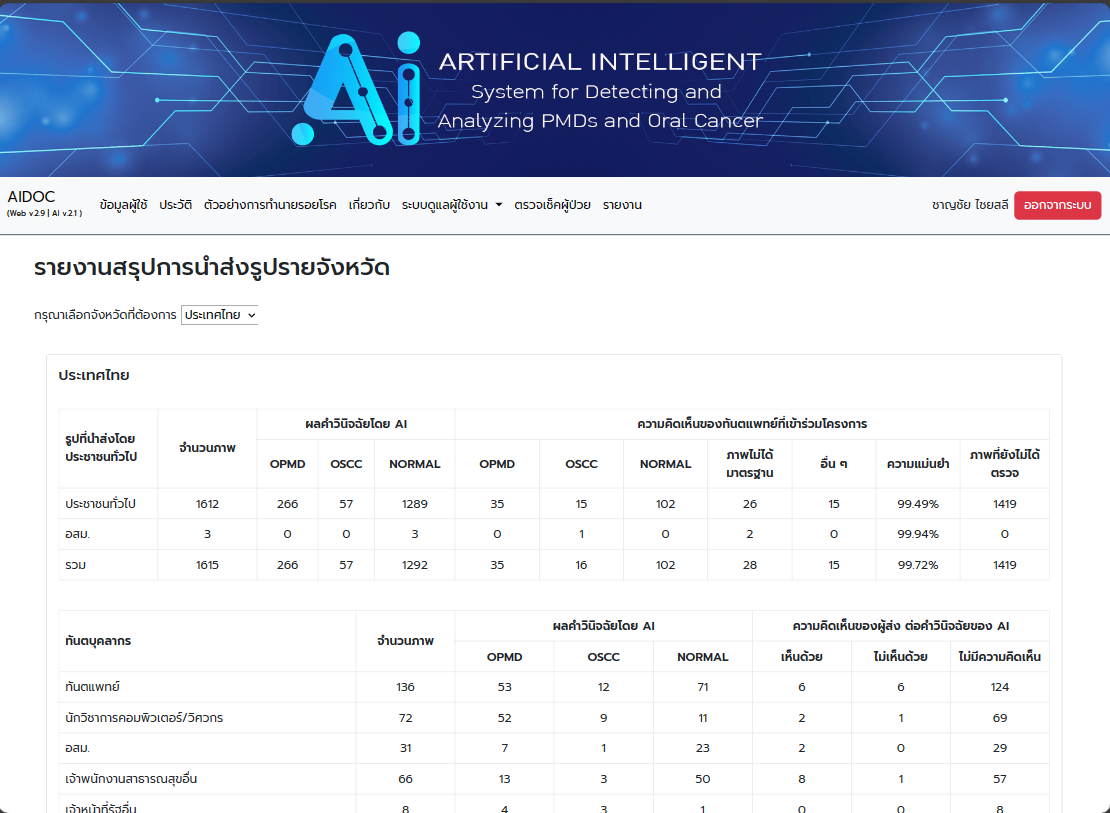
\includegraphics[scale=0.3]{report_user.png}
  \caption{report page}
  \label{fig:report_user}
\end{figure}

\subsection{ประชาชนทั่วไป (General public)}
\subsubsection{หน้าเข้าสู่ระบบ (Login Page)}
\begin{figure}[H]
  \centering
  \graphicspath{{./images/}}
  
\includegraphics[scale=0.3]{login_patient.png}
  \caption{login page}
  \label{fig:login_patient}
\end{figure}

\subsubsection{หน้าลงทะเบียน (Register Page)}
\begin{figure}[H]
  \centering
  \graphicspath{{./images/}}
  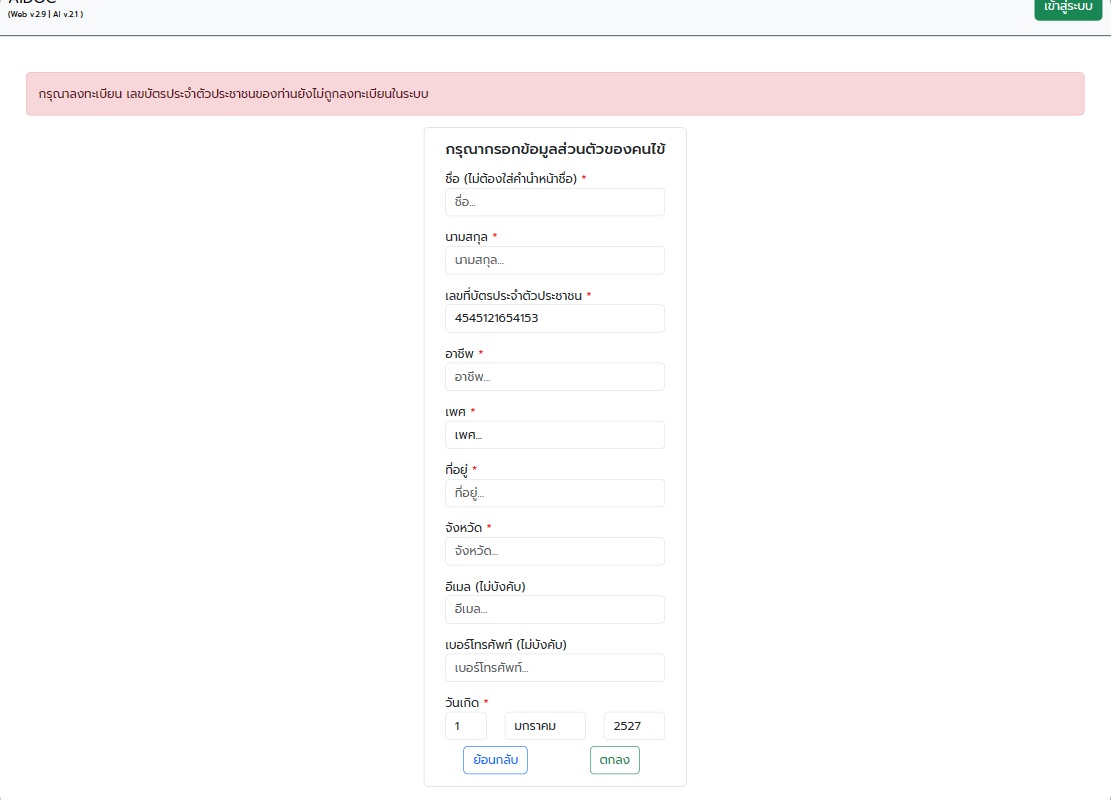
\includegraphics[scale=0.3]{register_patient.png}
  \caption{register page}
  \label{fig:register_patient}
\end{figure}

\subsubsection{หน้าอัพโหลดรูปภาพ (Upload Page)}

\begin{figure}[H]
  \centering
  \graphicspath{{./images/}}
  
\includegraphics[scale=0.3]{upload_patient.png}
  \caption{upload page}
  \label{fig:upload_patient}
\end{figure}

  \begin{figure}[H]
    \centering
    \graphicspath{{./images/}}
    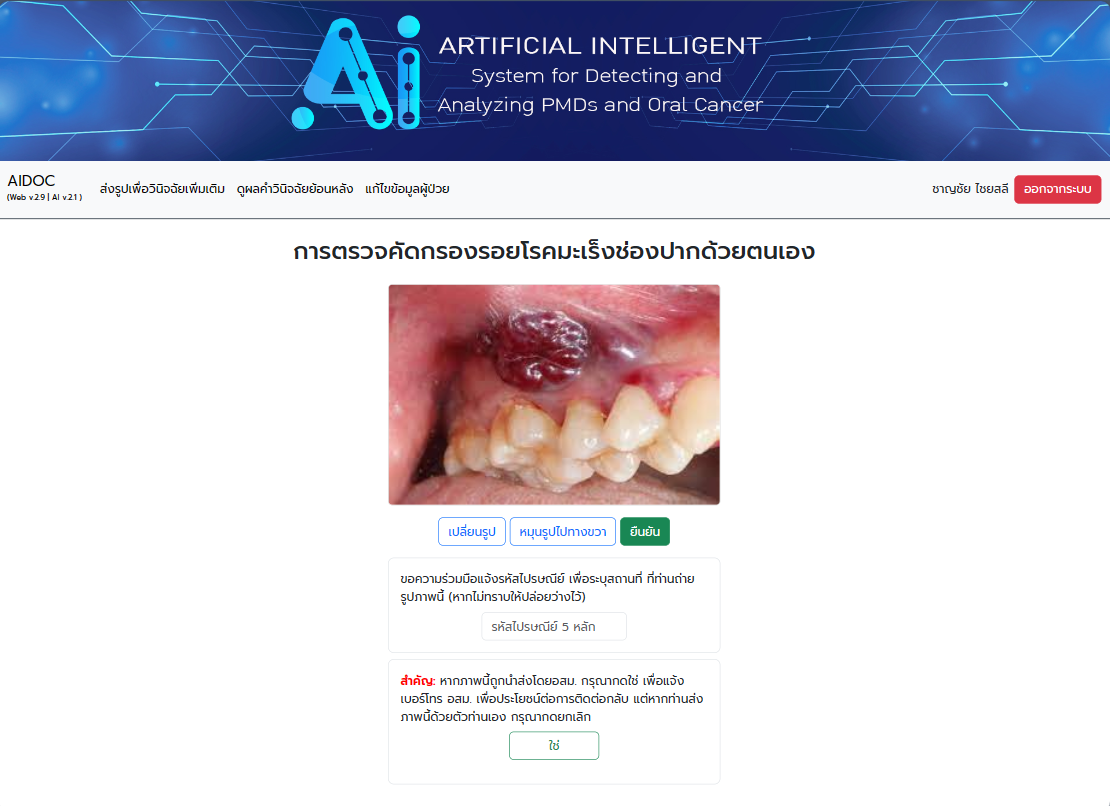
\includegraphics[scale=0.3]{preview_patient.png}
    \caption{preview page}
    \label{fig:preview_patient}
  \end{figure}
    \begin{figure}[H]
      \centering
      \graphicspath{{./images/}}
      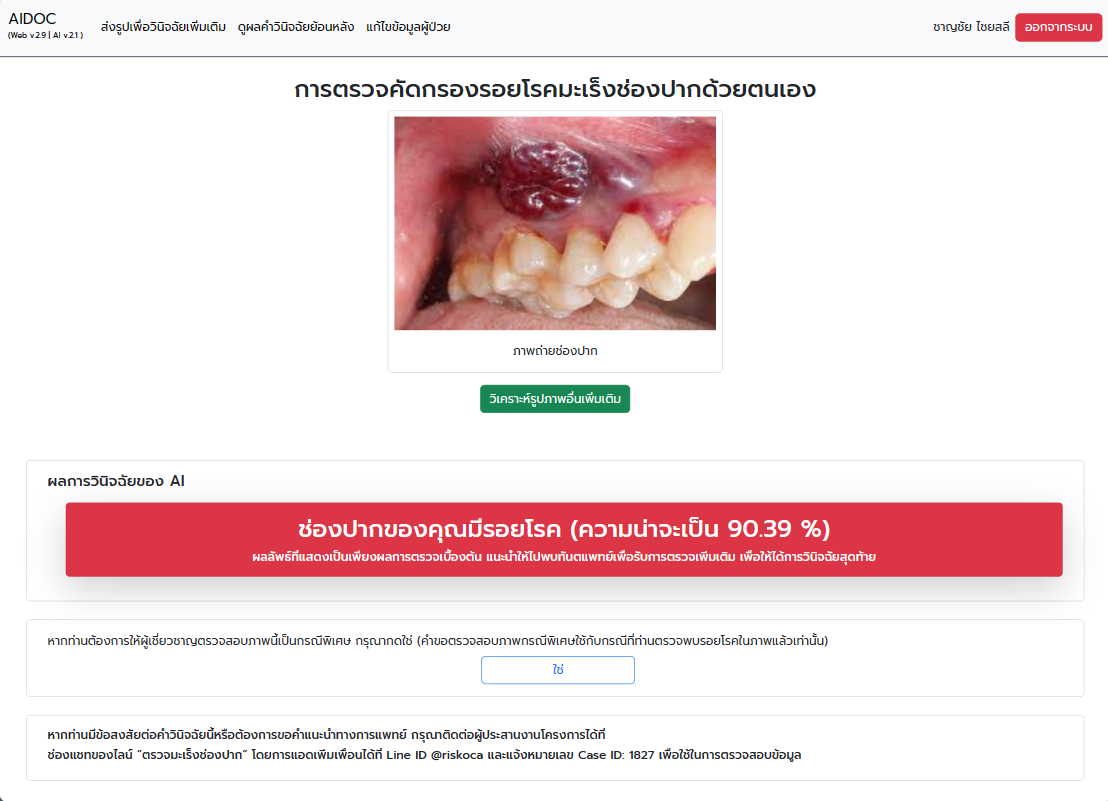
\includegraphics[scale=0.3]{upload_complete_patient.png}
      \caption{uploaded page}
      \label{fig:upload_complete_patient}
    \end{figure}

\subsection{อาสาสมัครสาธารณสุขประจําหมู่บ้าน (อสม.)}
\subsubsection{หน้าเข้าสู่ระบบ (Login Page)}
\begin{figure}[H]
  \centering
  \graphicspath{{./images/}}
  
\includegraphics[scale=0.3]{login_volunteer.png}
  \caption{login page}
  \label{fig:login_volunteer}
\end{figure}

\subsubsection{หน้าลงทะเบียน (Register Page)}
\begin{figure}[H]
  \centering
  \graphicspath{{./images/}}
  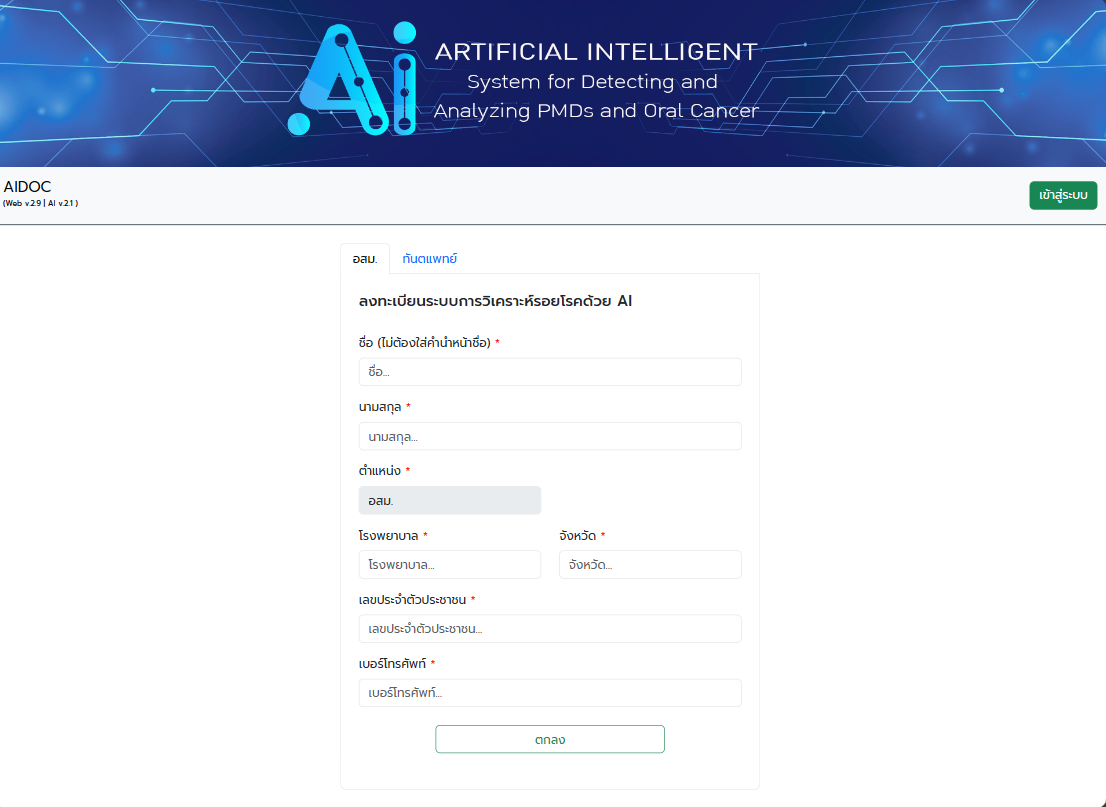
\includegraphics[scale=0.3]{register_volunteer.png}
  \caption{register page}
  \label{fig:register_volunteer}
\end{figure}

\subsubsection{หน้าประวัติการอัพโหลดรูปภาพ (History Page)}

\begin{figure}[H]
  \centering
  \graphicspath{{./images/}}
  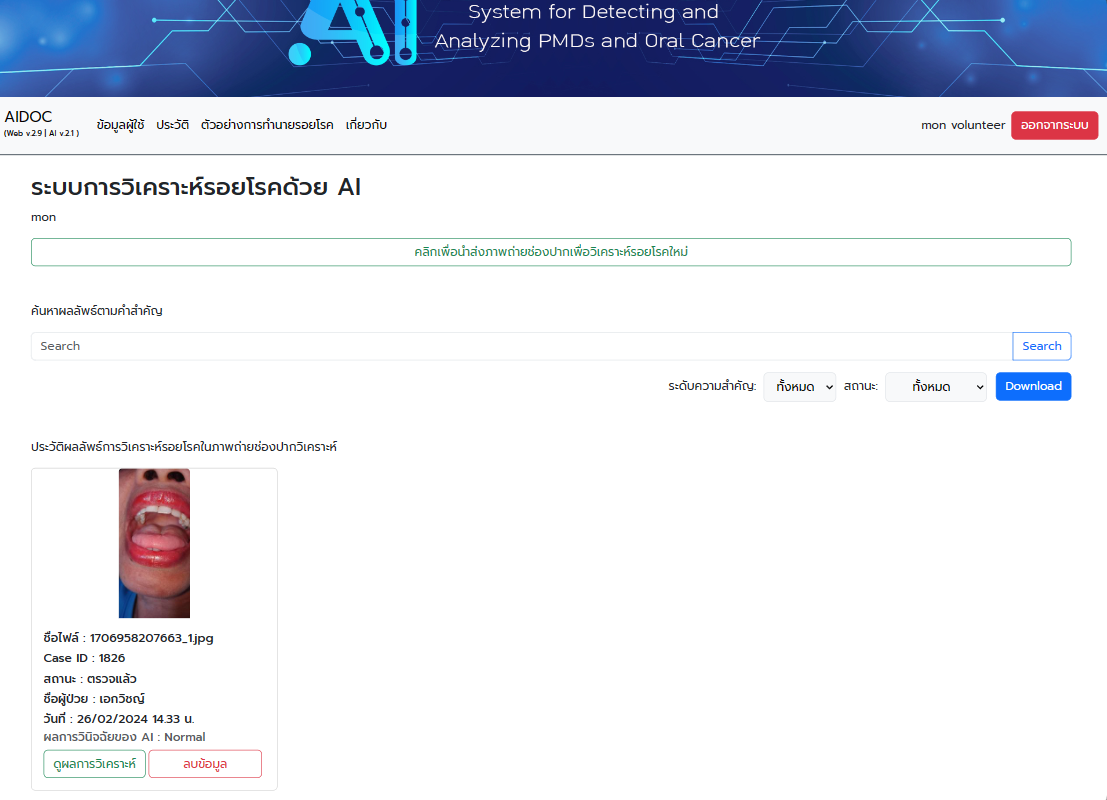
\includegraphics[scale=0.3]{history_volunteer.png}
  \caption{history page}
  \label{fig:history_volunteer}
\end{figure}

\subsubsection{หน้าอัพโหลดรูปภาพ (Upload Page)}
\begin{figure}[H]
  \centering
  \graphicspath{{./images/}}
  
\includegraphics[scale=0.3]{upload_volunteer.png}
  \caption{upload page}
  \label{fig:upload_volunteer}
\end{figure}

  \begin{figure}[H]
    \centering
    \graphicspath{{./images/}}
    
\includegraphics[scale=0.3]{preview_volunteer.png}
    \caption{preview page}
    \label{fig:preview_volunteer}
  \end{figure}

    \begin{figure}[H]
      \centering
      \graphicspath{{./images/}}
      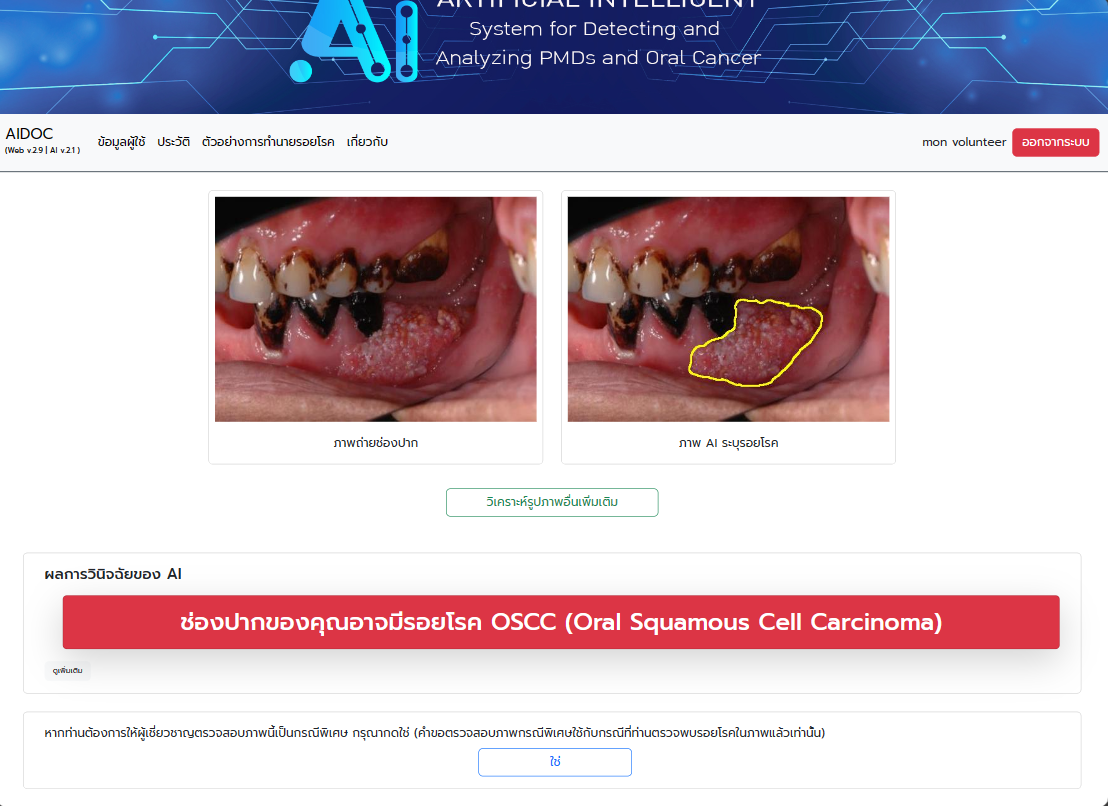
\includegraphics[scale=0.3]{upload_complete_volunteer.png}
      \caption{uploaded page}
      \label{fig:upload_complete_volunteer}
    \end{figure}